\begin{frame}{Extending an LLM with Vision: The Blueprint}
  \begingroup\centering
  \resizebox{\textwidth}{!}{%
  \begin{tikzpicture}[font=\sffamily\scriptsize, >=latex,
      box/.style={draw, rounded corners=0.1cm, align=center, minimum height=0.7cm},
      inp/.style={box, fill=gray!8, text width=1.9cm},
      enc/.style={box, fill=blue!12, text width=2.3cm},
      tkz/.style={box, fill=gray!15, text width=2.3cm},
      con/.style={box, fill=orange!16, text width=1.7cm},
      llm/.style={box, fill=green!14, text width=1.7cm, minimum height=1.9cm},
      vt/.style={draw, fill=blue!30, minimum size=0.3cm, inner sep=0pt},
      tt/.style={draw, fill=gray!30, minimum size=0.3cm, inner sep=0pt},
      num/.style={circle, fill=KAred, text=white, font=\sffamily\tiny\bfseries, inner sep=0pt, minimum size=0.34cm},
      arr/.style={->, thick}]
    \node[inp] (img) at (1.0,1.1)  {image, e.g.\\$336 \times 336$ px};
    \node[inp] (txt) at (1.0,-0.1) {text prompt\\``What does the\\sign say?''};
    \node[enc] (enc) at (3.65,1.1) {vision encoder\\(a ViT, CLIP- or\\SigLIP-trained)};
    \node[tkz] (tok) at (3.65,-0.1) {tokenizer +\\embedding table};
    \node[con] (con) at (6.15,1.1) {connector\\(projector or\\resampler)};
    \foreach \pk in {0,1,2,3} {
      \node[vt] at (7.75+0.35*\pk,0.5) {};
      \node[tt] at (9.15+0.35*\pk,0.5) {};
    }
    \node[llm] (llm) at (11.55,0.5) {decoder-only\\LLM};
    \node[align=center] (ans) at (13.4,0.5) {answer\\tokens};
    \draw[arr] (img) -- (enc);
    \draw[arr] (txt) -- (tok);
    \draw[arr] (enc) -- (con);
    \draw[arr] (con.east) -| (8.275,0.65);
    \draw[arr] (tok.east) -| (9.675,0.35);
    \draw[arr] (10.35,0.5) -- (llm.west);
    \draw[arr] (llm) -- (ans);
    \node[num] at (enc.north east) {1};
    \node[num] at (con.north east) {2};
    \node[num] at (llm.north west) {3};
    \node[num] at (7.32,0.5) {4};
  \end{tikzpicture}}\\[0.2em]
  {\scriptsize Blue: visual tokens; gray: text tokens; red: the four design decisions. The tokenizer splits text into subword units, which the embedding table maps to vectors.\par}
  \endgroup
  \vspace{0.2em}
  \begin{columns}[T,onlytextwidth]
    \column{0.44\textwidth}
      \begin{itemize}\scriptsize\itemsep0.3em
        \item \textbf{Training signal:} predict the next text token, given the image and the text before it:
        \[ \mathcal{L}(\theta) = -\sum\nolimits_{i \in \mathcal{A}} \log p_{\theta}\big(x_i \mid \mathbf{H}_v,\, x_{<i}\big) \]
        $\mathbf{H}_v$: visual tokens, as in LLaVA; $x_{<i}$: earlier text tokens; $\mathcal{A}$: positions that carry loss (the answer tokens in LLaVA's instruction tuning, all text tokens in Flamingo's pretraining); $\theta$: the unfrozen weights, connector included.
      \end{itemize}
    \column{0.54\textwidth}
      \begin{enumerate}\scriptsize\itemsep0.15em
        \item \textbf{Encoder:} which ViT, trained how, at what resolution.
        \item \textbf{Connector:} projector or learned-query resampler.
        \item \textbf{Entry point:} input sequence or cross-attention.
        \item \textbf{Token budget:} visual tokens per image.
      \end{enumerate}
      \vspace{0.2em}
      {\scriptsize BLIP-2 (Q-Former, input sequence), Flamingo (Perceiver Resampler, cross-attention) and LLaVA (projector, input sequence) are three settings of decisions 2 and 3.\par}
  \end{columns}
\end{frame}

\begin{frame}{Where Vision Enters: Tokens or Cross-Attention}
  \begin{columns}[T,onlytextwidth]
    \column{0.49\textwidth}
      {\footnotesize\textbf{(a) Visual tokens in the input sequence}\par}
      \vspace{0.1em}
      \begingroup\centering
      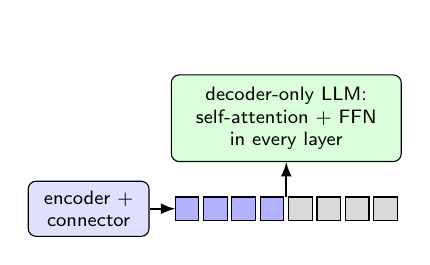
\begin{tikzpicture}[font=\sffamily\scriptsize, >=latex,
          box/.style={draw, rounded corners=0.1cm, align=center},
          vt/.style={draw, fill=blue!30, minimum size=0.3cm, inner sep=0pt},
          tt/.style={draw, fill=gray!30, minimum size=0.3cm, inner sep=0pt},
          arr/.style={->, thick}]
        \path (0,2.55);
        \node[box, fill=blue!12, text width=1.3cm, minimum height=0.7cm] (ea) at (0.75,0.25) {encoder +\\connector};
        \foreach \pk in {0,1,2,3} {
          \node[vt] at (2.0+0.36*\pk,0.25) {};
          \node[tt] at (3.44+0.36*\pk,0.25) {};
        }
        \node[box, fill=green!14, minimum width=2.92cm, minimum height=1.1cm] (la) at (3.26,1.4) {decoder-only LLM:\\self-attention + FFN\\in every layer};
        \draw[arr] (ea.east) -- (1.85,0.25);
        \draw[arr] (3.26,0.4) -- (la.south);
      \end{tikzpicture}\par
      \endgroup
      \begin{itemize}\scriptsize\itemsep0.3em
        \item \textbf{Used by} LLaVA, BLIP-2 (Q-Former outputs prepended as ``soft visual prompts'') and Qwen-VL (256 tokens between \texttt{<img>} and \texttt{</img>}). No new LLM layers; the LLM may stay frozen (BLIP-2) or be tuned (LLaVA).
        \item \textbf{Cost:} every visual token takes a context position and passes through self-attention and the FFN (the per-token MLP of each block, FFW in Flamingo's figures) in every layer.
      \end{itemize}
    \column{0.49\textwidth}
      {\footnotesize\textbf{(b) Cross-attention layers inside the LLM}\par}
      \vspace{0.1em}
      \begingroup\centering
      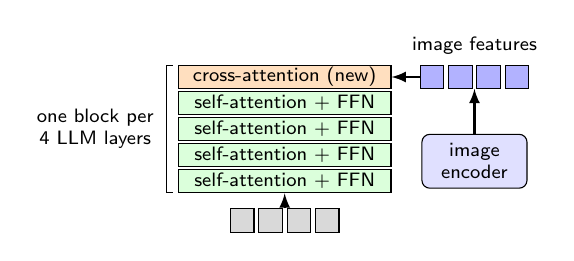
\begin{tikzpicture}[font=\sffamily\scriptsize, >=latex,
          box/.style={draw, rounded corners=0.1cm, align=center},
          lay/.style={draw, minimum width=2.7cm, minimum height=0.3cm, inner sep=0pt},
          vt/.style={draw, fill=blue!30, minimum size=0.3cm, inner sep=0pt},
          tt/.style={draw, fill=gray!30, minimum size=0.3cm, inner sep=0pt},
          arr/.style={->, thick}]
        \foreach \pk in {0,1,2,3} {
          \node[tt] at (1.94+0.36*\pk,0.2) {};
          \node[vt] at (4.35+0.36*\pk,2.02) {};
        }
        \node[lay, fill=green!14] (l1) at (2.48,0.70) {self-attention + FFN};
        \node[lay, fill=green!14] at (2.48,1.03) {self-attention + FFN};
        \node[lay, fill=green!14] at (2.48,1.36) {self-attention + FFN};
        \node[lay, fill=green!14] at (2.48,1.69) {self-attention + FFN};
        \node[lay, fill=orange!25] (xa) at (2.48,2.02) {cross-attention (new)};
        \draw (1.06,0.55) -- (0.98,0.55) -- (0.98,2.17) -- (1.06,2.17);
        \node[anchor=east, align=center] at (0.94,1.36) {one block per\\4 LLM layers};
        \node[box, fill=blue!12, text width=1.1cm, minimum height=0.6cm] (eb) at (4.89,0.95) {image\\encoder};
        \draw[arr] (2.48,0.35) -- (l1.south);
        \draw[arr] (4.2,2.02) -- (xa.east);
        \draw[arr] (eb.north) -- (4.89,1.87);
        \node at (4.89,2.42) {image features};
      \end{tikzpicture}\par
      \endgroup
      \begin{itemize}\scriptsize\itemsep0.3em
        \item \textbf{Used by} Flamingo (every 7th layer in Flamingo-80B) and Meta's Llama 3 (every 4th, as drawn). Text tokens query the image features: the sequence keeps its length, and image tokens skip the LLM's FFNs.
        \item \textbf{Cost:} new weights, about 100B in the cross-attention layers of the 405B Llama 3. The LLM can stay frozen; Llama 3 freezes it ``to maintain text-only performance''.
      \end{itemize}
  \end{columns}
  \vspace{0.2em}
  {\scriptsize Llama 3 feeds speech in by route (a) and vision by route (b). Sources: Llama Team, AI @ Meta, ``The Llama 3 Herd of Models,'' 2024, \href{https://arxiv.org/abs/2407.21783v3}{arXiv:2407.21783v3}, Sec.~7, 7.2, 7.5.2, 8.2.1; BLIP-2, \href{https://arxiv.org/abs/2301.12597v3}{arXiv:2301.12597v3}, Sec.~3.3; Qwen-VL, \href{https://arxiv.org/abs/2308.12966v3}{arXiv:2308.12966v3}, Sec.~2.1--2.2; Flamingo, \href{https://arxiv.org/abs/2204.14198v2}{arXiv:2204.14198v2}, Sec.~3.3.\par}
\end{frame}

\begin{frame}{Choosing the Connector}
  \begingroup\centering
  {\scriptsize\setlength{\tabcolsep}{4pt}
  \begin{tabular}{>{\raggedright\arraybackslash}p{3.0cm} >{\raggedright\arraybackslash}p{2.6cm} >{\raggedright\arraybackslash}p{1.8cm} >{\raggedright\arraybackslash}p{4.8cm}}
    \toprule
    \textbf{Connector} & \textbf{Tokens per image} & \textbf{Example} & \textbf{What it trades} \\
    \midrule
    Linear projection & 256 at 224 px & LLaVA & one per patch; keeps local detail \\
    \addlinespace[0.2em]
    Two-layer MLP & 576 at 336 px & LLaVA-1.5 & one per patch; more capacity \\
    \addlinespace[0.2em]
    Q-Former & 32 learned queries & BLIP-2 & fixed and short; own pretraining \\
    \addlinespace[0.2em]
    Perceiver Resampler & 64 learned latents & Flamingo & fixed at any resolution or frame count \\
    \addlinespace[0.2em]
    Cross-attention resampler & 256 from 1,024 patches & Qwen-VL & one layer; 2D position encodings limit layout loss \\
    \addlinespace[0.2em]
    Pixel unshuffle + MLP & 256 per 448-px tile & InternVL 1.5 & folds $32 \times 32$ patch features into $16 \times 16$ vectors with $4\times$ the channels (the paper calls it pixel shuffle); count grows with the tiles \\
    \addlinespace[0.2em]
    $2 \times 2$ merge + MLP & one per $28 \times 28$ px & Qwen2-VL & an MLP merges each $2 \times 2$ group; count follows the image area \\
    \bottomrule
  \end{tabular}\par}
  \endgroup
  \vspace{0.4em}
  \begin{itemize}\scriptsize\itemsep0.2em
    \item \textbf{Two properties a connector needs} (Honeybee, Cha et al., CVPR 2024): ``flexibility in managing the number of visual tokens'', which learned-query resamplers have, and ``preservation of local context from visual features'', which per-patch projectors have. $2 \times 2$ folding sits between them: a fixed $4\times$ cut that keeps each block's neighbours together.
  \end{itemize}
  \vspace{0.1em}
  {\scriptsize Sources: Qwen-VL, \href{https://arxiv.org/abs/2308.12966v3}{arXiv:2308.12966v3}, Sec.~2.1, App.~E.2; InternVL 1.5, \href{https://arxiv.org/abs/2404.16821v2}{arXiv:2404.16821v2}, Sec.~3.1, and released code; Qwen2-VL, \href{https://arxiv.org/abs/2409.12191v2}{arXiv:2409.12191v2}, Sec.~2.1; Cha et al., ``Honeybee: Locality-enhanced Projector for Multimodal LLM,'' CVPR 2024, \href{https://arxiv.org/abs/2312.06742v2}{arXiv:2312.06742v2}, abstract and Fig.~2.\par}
\end{frame}

\begin{frame}{What the Ablations Say: Encoder and Connector}
  \begingroup\centering
  {\scriptsize\setlength{\tabcolsep}{4pt}
  \begin{tabular}{@{}l ccc ccc ccc@{}}
    \toprule
     & \multicolumn{3}{c}{0-shot} & \multicolumn{3}{c}{4-shot} & \multicolumn{3}{c}{8-shot} \\
    \cmidrule(lr){2-4}\cmidrule(lr){5-7}\cmidrule(l){8-10}
    Image size, tokens & Avg & Att & C-Abs & Avg & Att & C-Abs & Avg & Att & C-Abs \\
    \midrule
    224 px, 64 & 30.9 & 30.2 & 30.7 & 55.5 & 52.8 & 55.0 & 58.7 & 56.9 & 62.5 \\
    336 px, 64 & 31.9 & 30.4 & 31.7 & 57.0 & 56.0 & 58.7 & 57.9 & 61.1 & 62.0 \\
    336 px, 144 & 32.2 & 31.5 & 33.4 & 59.1 & 58.2 & 57.4 & 58.7 & 62.3 & 61.2 \\
    \bottomrule
  \end{tabular}\par}
  \vspace{0.2em}
  {\scriptsize Average over 8 captioning and VQA benchmarks. Avg / Att: average / attention pooling; C-Abs: C-Abstractor. Encoder (CLIP-trained ViT-L/14) and 1.2B LLM fixed; connector, image size and token count varied. Values from McKinzie et al., ``MM1: Methods, Analysis \& Insights from Multimodal LLM Pre-training,'' 2024, \href{https://arxiv.org/abs/2403.09611v4}{arXiv:2403.09611v4}, Figure~4; Sections~3.1--3.2 and~4.\par}
  \endgroup
  \vspace{0.2em}
  \begin{itemize}\scriptsize\itemsep0.25em
    \item \textbf{Connector lesson:} ``Number of visual tokens and image resolution matters most, while the type of VL connector has little effect.'' Average pooling, attention pooling with learned queries and C-Abstractor (ResNet blocks with adaptive pooling, from Honeybee) ``achieve very similar results at the 336px and 144 token setting'' after instruction tuning.
    \item \textbf{Encoder lesson} (with a 2.9B LLM, Table~1): ``Image resolution has the highest impact, followed by model size and training data composition'': 224 to 336 px gave about 3\% on all metrics, ViT-L to ViT-H (Huge, twice the parameters) usually less than 1\%. The final MM1 uses a ViT-H at 378 px and 144 tokens.
    \item \textbf{Cambrian-1} (Tong et al., NeurIPS 2024, \href{https://arxiv.org/abs/2406.16860v2}{arXiv:2406.16860v2}, Sec.~3.4) compared over 20 vision encoders: ``Language supervision offers strong advantages, but the performance gap can be narrowed with SSL methods given enough data and proper tuning'' (SSL: self-supervised learning, such as DINOv2).
  \end{itemize}
\end{frame}

\begin{frame}{What the Ablations Say: Pretraining Data}
  \begin{columns}[T,onlytextwidth]
    \column{0.53\textwidth}
      \begin{itemize}\scriptsize\itemsep0.35em
        \item \textbf{Three kinds of data:} image-caption pairs (short text, closely tied to the image); interleaved image-text web documents (longer, more varied text, more loosely tied to the images, as in Flamingo); and text-only data, which preserves the LLM's language skills.
        \item \textbf{Data lesson 1:} ``Interleaved data is instrumental for few-shot and text-only performance, while captioning data lifts zero-shot performance.'' Zero-shot rises from 25.8 with no captions to 39.3 with captions only; 8-shot falls from 62.2 at 50/50 to 45 with captions only.
        \item \textbf{Why:} an interleaved page already looks like a few-shot prompt, with several related images and texts in one sequence. The authors add a caveat: 3 of the 8 benchmarks are captioning, which favors caption data at zero shot.
        \item \textbf{Lessons 2 and 3:} text-only data lifts text-only scores, and few-shot scores when mixed with captions (with interleaved data they dip slightly); a caption/interleaved/text ratio of 5:5:1 gave strong multimodal results with comparable text-only scores.
        \item \textbf{Final MM1 mix:} 45\% interleaved documents, 45\% image-caption pairs, 10\% text-only.
      \end{itemize}
    \column{0.45\textwidth}
      \centering
      \vspace{0.2em}
      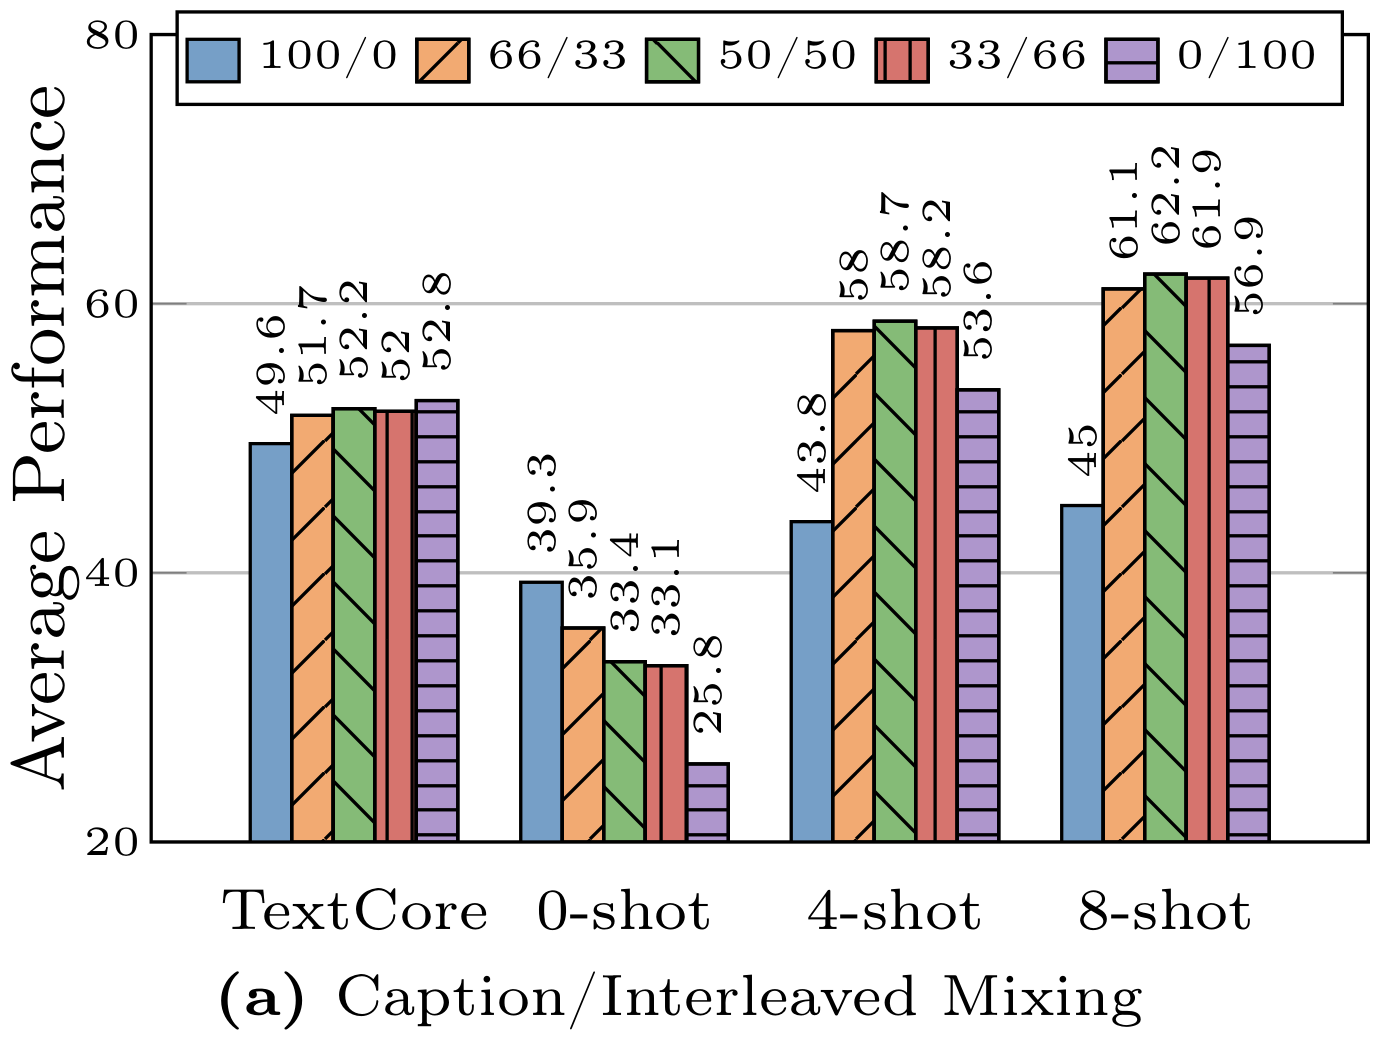
\includegraphics[width=\linewidth,height=0.56\textheight,keepaspectratio]{images/vision-language-models/mm1_fig5a_caption_interleaved_mix.png}\\[0.2em]
      {\scriptsize Legend: caption/interleaved share of the image data (100/0: captions only). TextCore: average over 8 text-only tasks. McKinzie et al., \href{https://arxiv.org/abs/2403.09611v4}{arXiv:2403.09611v4}, Figure~5(a) and Section~3.3.\par}
  \end{columns}
\end{frame}

\begin{frame}{Counting Visual Tokens: A Worked Example}
  \begingroup\scriptsize
  A ViT with 14-pixel patches gives $(s/14)^2$ tokens for an $s \times s$ image: 256 at 224 px, 576 at 336 px, 2,304 at 672 px.\par
  \endgroup
  \vspace{0.2em}
  \begingroup\centering
  {\scriptsize\setlength{\tabcolsep}{5pt}
  \begin{tabular}{>{\raggedright\arraybackslash}p{2.6cm} >{\raggedright\arraybackslash}p{8.2cm} r}
    \toprule
    \textbf{One $1344 \times 1344$ photo} & \textbf{How the count arises} & \textbf{Visual tokens} \\
    \midrule
    BLIP-2 & 32 Q-Former queries at any input resolution (224 px in pretraining) & 32 \\
    Flamingo & 64 Perceiver Resampler latents, read through cross-attention & 64 \\
    Qwen-VL & 256 learned queries; the image is resized to $448 \times 448$ & 256 \\
    LLaVA-1.5 & $(336/14)^2 = 24^2$; the image is resized to $336 \times 336$ & 576 \\
    LLaVA-NeXT (AnyRes) & $4 \times 576 + 576$: $2 \times 2$ tiles of 336 px plus the whole image at 336 px & 2,880 \\
    InternVL 1.5 & $(9 + 1) \times 256$: $3 \times 3$ tiles of 448 px plus a thumbnail (default 12-tile cap) & 2,560 \\
    Qwen2-VL & $(1344/28)^2 = 48^2$: the full image at native resolution & 2,304 \\
    \bottomrule
  \end{tabular}\par}
  \endgroup
  \vspace{0.15em}
  \begin{itemize}\scriptsize\itemsep0.2em
    \item \textbf{Attention grows with the square.} From 576 to 2,880 visual tokens, the visual block of each head's score matrix grows from $576^2 = 331{,}776$ to $2{,}880^2 = 8{,}294{,}400$ entries (a causal mask uses about half), $(2{,}880/576)^2 = 25$ times. Per-token costs (FFN, stored keys and values) grow 5 times.
    \item \textbf{Images and frames add up.} Eight video frames at 576 tokens need 4,608 tokens, more than Vicuna v1.5's 4,096-token context; Qwen2-VL caps a training video at 16,384 tokens by lowering frame resolution.
    \item \textbf{Cross-attention moves the cost.} In Llama 3's image training, an image has 2,308 tokens and its text 192 on average; the image tokens pass only through the image encoder and the cross-attention layers.
  \end{itemize}
  \vspace{0.1em}
  {\scriptsize Counts leave out delimiter and row-end tokens. Sources: InternVL 1.5, \href{https://arxiv.org/abs/2404.16821v2}{arXiv:2404.16821v2}, Sec.~3.3, and released code; Qwen2-VL, \href{https://arxiv.org/abs/2409.12191v2}{arXiv:2409.12191v2}, Sec.~2.1; Llama 3, \href{https://arxiv.org/abs/2407.21783v3}{arXiv:2407.21783v3}, Sec.~7.3.\par}
\end{frame}
